\documentclass[11pt]{article}
\usepackage[final]{acl2023}
\usepackage{times}
\usepackage{latexsym}
\usepackage{amsmath,amssymb,booktabs,graphicx,float,placeins}
\usepackage{colortbl}
\usepackage[T1]{fontenc}
\usepackage[utf8]{inputenc}
\usepackage{microtype}
\title{Talk Like a Structured Graph? Structural Statistics Help Small LLMs\\Mainly by Stating the Answer}
\author{
  Inbal Moryles\\
  \footnotesize\texttt{github.com/iinbal}\\
  \footnotesize\texttt{inbalmoryles@tau.ac.il}
  \And
  Gal Barak\\
  \footnotesize\texttt{github.com/GalBrk}\\
  \footnotesize\texttt{galbarak2@mail.tau.ac.il}
  \And
  Nitzan Zacharia\\
  \footnotesize\texttt{github.com/NitzanZacharia}\\
  \footnotesize\texttt{zacharia1@mail.tau.ac.il}
}
\date{}
\begin{document}
\raggedbottom
\maketitle
\begin{abstract}
Graph models gain from structural encodings such as node degree and random-walk return probabilities. We ask whether a frozen language model reading a graph as text gains when the same statistics are written as sentences in a \emph{primer} before GraphQA's incident encoding. In paired tests at several edge densities, for two model sizes with thinking off and on, we compare each primer with no primer, a structure-free filler and the model's thinking mode. Mostly, statistics do not improve how the model computes; they help by stating the answer. Stated degrees raise node-degree accuracy by $7.5$ to $12.2$ points where a model counts unreliably, and cost the one model that already counts correctly $6.5$ to $8.0$. Other statistics have mostly small, model-dependent effects and often change the same answers as the filler. They narrow the gap to thinking without closing it, except one sentence that makes the model restate the queried node's line, matching thinking on one task. With thinking on, models check stated values against their own count, and much of a primer's effect is on finishing within the budget. Accuracy can also mislead: without thinking, stated degrees can lower cycle-detection accuracy yet raise the share of validly argued answers. % [main] [overlap] [vsthink] [churnwhy] [ccvalid]
\end{abstract}

\section{Introduction}
\label{sec:intro}
Structural encodings, such as node degree and random-walk return probabilities, are a standard ingredient of graph neural networks and graph Transformers \citep{dwivedi2022graph,rampasek2022recipe}. A language model that reads a graph as text must instead recover such quantities itself, and its accuracy depends on how the graph is written \citep{fatemi2023talklikeagraph,wang2023nlgraph}. Statistics are cheap to precompute, so an obvious aid is to state them in the prompt. We ask: \emph{when a frozen language model reads a textual graph, do explicit structural statistics improve execution of graph queries?} By \emph{execution} we mean computing the answer from the graph's edges, not copying it from elsewhere in the prompt.

A primer can raise accuracy by stating the answer, by adding information that narrows it, or by changing how the model reads the graph; only the last is better execution. In an Erd\H{o}s-R\'enyi graph every edge is independent of the others, so beyond a node's degree, clustering and return probabilities carry almost no information about GraphQA's answers (\S\ref{sec:states}). A gain from them therefore reflects how the model reads the prompt, not new information. We measure each primer's effect in both modes against three references: no primer; a structure-free \emph{filler}, for what added text does on its own; and, for the plain mode, the same model thinking without a primer. The last asks whether a preamble can stand in for reasoning that costs $6$-$17$ times the output tokens on node degree. The degree primer, which states the answer to node-degree and edge-count queries, is a positive control. % [ddgap]

Specifically: does a primer that states the answer help, and where? Do statistics that do not state it help beyond what any added text does? Can a primer bring a model's plain mode level with its thinking mode? And do the responses show the primer being used? In short, explicit statistics mostly do not improve execution. A stated answer helps where the model's own count is unreliable and hurts where it is reliable. Other statistics have mostly small effects whose sign depends on the model. One sentence that changes the procedure matches thinking, on one task. Responses show stated values being used, but not other statistics.

\section{Related Work}
\label{sec:related}
\paragraph{Graphs as text.} GraphQA \citep{fatemi2023talklikeagraph} and NLGraph \citep{wang2023nlgraph} show that LLM accuracy on graph queries depends on encoding, task and graph structure, and NLGraph's build-a-graph and algorithmic prompts change the procedure by instruction. We keep GraphQA's tasks and encoding and change only a preamble.

\paragraph{Structure for LLMs.} Structure can be passed as learned soft tokens \citep{perozzi2024letyourgraph} or as motif descriptions, which help on some tasks \citep{das2024modality}. Structural descriptions in a prompt, however, need not be read as topology \citep{huang2024can}. We state the encodings of graph learning as sentences to a frozen model and control for what they state.

\paragraph{Controls and faithfulness.} Added or irrelevant text changes LLM answers \citep{shi2023distracted,levy2024sametask}, as does formatting \citep{sclar2024quantifying}. Partial-input baselines expose answers a dataset gives away \citep{feng2019misleading}, as our graph-blind solver does for primers. A right answer can rest on a wrong route \citep{geirhos2020shortcut}, and a model's stated reasoning need not reflect the computation behind it \citep{turpin2023unfaithful}, so we treat responses as claims to check.

\section{Method}
\label{sec:method}
\begin{figure}[!t]
\centering
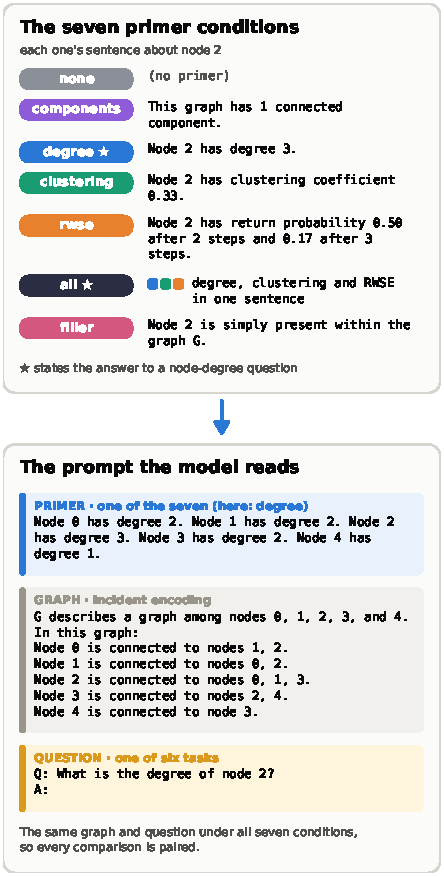
\includegraphics[width=0.82\columnwidth]{fig_primer_usage.pdf}
\caption{How a primer is used. Top: the seven conditions, each with its sentence about node~2 of a five-node example (the study's graphs have $40$ nodes); $\bigstar$ marks the two that state a node-degree answer. Bottom: the prompt the model reads, one primer followed by GraphQA's incident encoding and the question.}
\label{fig:prompt}
\end{figure}

\begin{table*}[t]
\centering\scriptsize
\setlength{\tabcolsep}{3.4pt}
\begin{tabular}{llrrrrrrr}
\toprule
Task & Arm & none & degree & clustering & RWSE & all & components & filler\\
\midrule
Degree & 1.7P & 60.50 & \cellcolor{black!12}$\mathbf{+7.5}^{\mathrm{f}}$ & $+3.0$ & $+4.0$ & \cellcolor{black!12}$\mathbf{+10.2}^{\mathrm{f}}$ & $+1.8$ & $-0.5$\\ % [main] [bars]
 & 1.7T & 76.25 & \cellcolor{black!12}$\mathbf{+8.8}^{\mathrm{f}}$ & $+1.5^{\mathrm{f}}$ & $+2.5^{\mathrm{f}}$ & \cellcolor{black!12}$\mathbf{+12.2}^{\mathrm{f}}$ & $-1.0$ & $-3.0$\\ % [main] [bars]
 & 4P & 99.25 & \cellcolor{black!12}$\mathbf{-6.5}^{\mathrm{f}}$ & $-0.5$ & $\mathbf{-2.2}$ & \cellcolor{black!12}$\mathbf{-8.0}^{\mathrm{f}}$ & $+0.2$ & $-0.5$\\ % [main] [bars]
 & 4T & 97.00 & \cellcolor{black!12}$+2.5$ & $+1.8$ & $-1.2^{\mathrm{f}}$ & \cellcolor{black!12}$+0.5$ & $+0.2$ & $+2.0$\\ % [main] [bars]
\addlinespace[2pt]
Neighbors & 1.7P & 72.50 & $+3.5^{\mathrm{f}}$ & $+1.2^{\mathrm{f}}$ & $+1.0^{\mathrm{f}}$ & $+2.0^{\mathrm{f}}$ & $+0.8^{\mathrm{f}}$ & $\mathbf{-6.2}$\\ % [main] [bars]
 & 1.7T & 78.75 & $\mathbf{+6.2}$ & $+2.0$ & $+0.2$ & $\mathbf{+6.2}$ & $+2.5$ & $+2.5$\\ % [main] [bars]
 & 4P & 86.00 & $-3.0^{\mathrm{f}}$ & $+1.0^{\mathrm{f}}$ & $+0.0^{\mathrm{f}}$ & $-2.8^{\mathrm{f}}$ & $\mathbf{+9.2}^{\mathrm{f}}$ & $\mathbf{-12.5}$\\ % [main] [bars]
 & 4T & 95.50 & $+0.5$ & $-0.8$ & $+0.5$ & $-1.2$ & $+0.5$ & $+1.2$\\ % [main] [bars]
\addlinespace[2pt]
Edge count & 1.7P & 1.25 & \cellcolor{black!12}$+3.0^{\dagger}$ & $-0.5^{\dagger}$ & $-0.8^{\dagger}$ & \cellcolor{black!12}$+0.8^{\dagger}$ & $-1.0^{\dagger}$ & $-0.5^{\dagger}$\\ % [main] [bars]
 & 1.7T & 15.75 & \cellcolor{black!12}$-3.2^{\dagger}$ & $-1.2^{\dagger}$ & $-3.2^{\dagger}$ & \cellcolor{black!12}$+5.0^{\dagger}$ & $-0.8^{\dagger}$ & $-1.5^{\dagger}$\\ % [main] [bars]
 & 4P & 2.00 & \cellcolor{black!12}$\mathbf{+27.2}^{\mathrm{f}}$ & $-1.2^{\mathrm{f}}$ & $-1.5^{\mathrm{f}}$ & \cellcolor{black!12}$\mathbf{+3.8}$ & $-1.2^{\mathrm{f}}$ & $+1.2$\\ % [main] [bars]
 & 4T & 20.00 & \cellcolor{black!12}$+8.5^{\dagger}$ & $+24.8^{\dagger}$ & $+10.2^{\dagger}$ & \cellcolor{black!12}$+1.8^{\dagger}$ & $+24.8^{\dagger}$ & $+12.2^{\dagger}$\\ % [main] [bars]
\addlinespace[2pt]
Edge exists & 1.7P & 70.50 & $+4.0^{\mathrm{f}}$ & $+3.8^{\mathrm{f}}$ & $+5.0^{\mathrm{f}}$ & $\mathbf{+11.5}^{\mathrm{f}}$ & $\mathbf{-8.2}^{\mathrm{f}}$ & $\mathbf{-15.8}$\\ % [main] [bars]
 & 1.7T & 99.00 & $-2.5$ & $-1.0$ & $-1.2$ & $-1.8$ & $-0.8$ & $-0.5$\\ % [main] [bars]
 & 4P & 90.50 & $\mathbf{-4.8}$ & $\mathbf{+4.0}^{\mathrm{f}}$ & $\mathbf{-10.0}$ & $\mathbf{-10.0}$ & $-2.8^{\mathrm{f}}$ & $\mathbf{-7.0}$\\ % [main] [bars]
 & 4T & 99.75 & $+0.0$ & $-0.8$ & $-1.2$ & $-1.0$ & $-0.5$ & $+0.0$\\ % [main] [bars]
\bottomrule
\end{tabular}
\caption{Primary result: correct share without a primer (\% of all prompts) and the paired change under each primer (points), on the same $400$ graphs per row ($p\leq.50$). Shaded: the primer states the answer. Bold: $q<.05$ against no primer (BH within arm, task and control); $^{\mathrm{f}}$: $q<.05$ against filler; $\dagger$: at least $15\%$ truncation on either side (unmarked). Intervals and the constant tasks: Table~\ref{tab:full}; truncation: Table~\ref{tab:truncmatrix}; balanced accuracy: Table~\ref{tab:ee}. P/T: plain/thinking.} % [setup] [main] [bars]
\label{tab:matrix}
\end{table*}

\paragraph{Models and graphs.} Qwen3-1.7B and Qwen3-4B \citep{qwen2025qwen3}, each with thinking off (plain, P) and on (T), make four \emph{arms}; decoding is zero-shot and greedy, one response per prompt (budgets in Appendix~\ref{app:audit}). A pilot on the published GraphQA graphs with Gemma~4 \citep{gemma4} and Qwen3-8B/14B left most arms near ceiling (Appendix~\ref{app:pilot}), and even at $40$ nodes Qwen3-8B answers $96.5$-$99.8\%$ of node-degree queries correctly. We therefore use harder graphs and smaller models, so that accuracy without a primer leaves room to measure a change in either direction. Our graphs are Erd\H{o}s-R\'enyi $G(n,p)$ \citep{erdosrenyi1959random} with $n=40$ at four edge densities up to $p=.50$ (the \emph{main sweep}) and, for node degree and edge existence, three more up to $p=.85$. Every condition and arm sees the same $100$ graphs per task and density, so every comparison is paired. % [setup] [fixdeg8]

\paragraph{Tasks.} GraphQA's six tasks in its incident encoding (Figure~\ref{fig:prompt}). Four have answers that vary: node degree, connected nodes (the queried node's neighbors, exact set match), edge count and edge existence. Two cannot measure reading at $40$ nodes: the encoding's first line lists all $40$ ids and every graph has a cycle, so node count is always $40$ and cycle check always yes (Appendix~\ref{app:more}). Cycle check serves only to ask what correct answers rest on. % [setup]

\paragraph{Primers and controls.} Before the encoding we place no primer, one sentence per node giving its degree, local clustering coefficient or return probabilities after 2 and 3 steps (RWSE; \citealp{dwivedi2022graph}), or \emph{all} three (Appendix~\ref{app:audit}). Two diagnostics follow the same format: a sentence giving the number of connected components, and the filler, which names every node and states no structure. The filler is about as long as the clustering primer, longer than degree and shorter than RWSE and all three (Appendix Table~\ref{tab:primerlength}). The graph-blind solver answers from the primer text alone.

\paragraph{Outcomes and statistics.} Each response is \emph{correct}, \emph{wrong} or \emph{truncated} (it used its whole budget); shares use all responses, and an effect is the paired change in the correct share, in points. Cells with at least $15\%$ truncation on either side are flagged ($\dagger$) and left out of pooled summaries. Edge existence is also scored by balanced accuracy, because the share of queried pairs that are edges rises from $10\%$ to $85\%$ with density. % [goldshare]
The primary analysis is Table~\ref{tab:matrix}: each primer against no primer and against filler on the same $400$ main-sweep graphs. It uses exact McNemar tests \citep{mcnemar1947note}, bootstrap intervals over graphs and Benjamini-Hochberg correction \citep{benjaminihochberg1995controlling} within each (arm, task, control) family; $q<.05$ is significant. Plain arms against thinking (Table~\ref{tab:vsthink}) use the same tests on the same graphs, and we call them equivalent when the $90\%$ interval of their difference lies within $\pm3$ points, about the 4B arms' median detectable gain. Analyses of mechanism are secondary and name their own test. Two limits of these tests matter for reading the results. \emph{Power:} over $400$ pairs the median detectable gain is $3.2$ to $5.7$ points, so a non-significant effect is unresolved, not zero (Appendix~\ref{app:audit}). % [lmde]
\emph{Noise:} generating the same prompts twice changes the outcome of $5.3\%$, so we compare net paired changes, never counts of changed answers. % [rerun]

\paragraph{Response readers.} Rule-based readers record whether a response reads a stated value off (a \emph{look-up}) or lists the neighbors, whether it reports a conflict with the primer, and which cycles and edges it asserts, checked against the graph. The conflict readers agree with blind hand labels on $90$-$100\%$ of items; the others were spot-checked by an LLM under human supervision (Appendix~\ref{app:audit}). % [dvc1] [dvc3] [dvc4] [dvc5] [dvc6]

\paragraph{Follow-ups.} Qwen3-1.7B node degree, plain and thinking, $400$ graphs per density at all seven densities, a fresh seed, and a $20$-$160$-node grid at mean degree $8$ and $16$ (also Qwen3-8B). % [ddplain] [ddrep] [fixdeg17]

\section{Results}
\label{sec:results}
\subsection{What each primer states}
\label{sec:states}
The graph-blind solver answers node degree and edge count perfectly from the degree primer or all three statistics, by reading the queried degree or halving the sum of the stated degrees. Every other primer barely informs it: at most $21.0\%$ on node degree, $10.4\%$ on edge count and $74.6\%$ on edge existence, against $14.4\%$, $3.0\%$ and $73.5\%$ with no primer (Appendix Table~\ref{tab:solver}). The shaded cells of Table~\ref{tab:matrix} are these answer-stating primers; we call every other cell a \emph{side} effect. % [bars]

\subsection{Stated answers are read off}
\label{sec:readoff}
\begin{figure}[t]
\centering
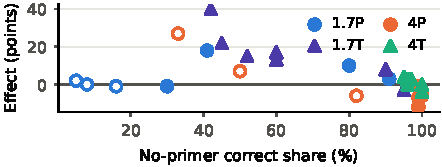
\includegraphics[width=\columnwidth]{fig_headroom.pdf}
\caption{The degree primer's effect on node degree against the no-primer correct share, per arm and density. Hollow: plain arm at $p\geq.65$ (smaller budget).} % [flip] [bands]
\label{fig:headroom}
\end{figure}

The degree primer raises node-degree accuracy for plain and thinking Qwen3-1.7B by $7.5$ and $8.8$ points and lowers it by $6.5$ for plain Qwen3-4B, which already counts correctly. % [main]
The gain is largest where a model is right about half the time and becomes a loss where it is right most of the time (Figure~\ref{fig:headroom}). % [plain17]
The same pattern holds within one model. The degree primer costs plain Qwen3-4B $11.8$ points on the queried nodes with the lowest degrees in their graph, and gains $10.6$ on those with the highest, which have the most neighbors to count. % [pdnode]

Reading a value off is itself fallible. Across all seven densities, where the answer is stated, plain Qwen3-1.7B gets it right only $43\%$ of the time. Plain Qwen3-4B stops listing the node's neighbors and reads the value off in $62\%$ of responses at $p=.50$. A third of its wrong look-ups copy the degree printed one sentence away, more often than chance predicts (Appendix~\ref{app:detail}). % [recover] [route] [copyerr]

\subsection{Side statistics have mostly small, model-dependent effects}
\label{sec:side}
Filler alone changes the outcome of $6.2$-$18.6\%$ of questions per arm, largely the same questions the primers change. Part of this is generation noise, though questions that flip on an identical rerun carry only a minority of each condition's changes (Appendix~\ref{app:detail}). We therefore compare each side effect with both controls as a net paired change. % [churn] [rerunflip]

Significant side effects differ in sign across statistics and models. On plain Qwen3-4B's edge existence, clustering raises balanced accuracy and RWSE lowers it ($q\leq.018$). All three statistics raise plain Qwen3-1.7B's by $7.8$ points but lower plain Qwen3-4B's by $6.5$ (Appendix Table~\ref{tab:ee}). % [eemain]
The largest side gain without the truncation flag, $+9.2$ on plain Qwen3-4B's neighbor sets, comes from the component sentence, which is the same for every connected graph. With it the model restates the queried node's line in nearly every response ($98.5\%$, against $63.0\%$): a change of procedure without information. % [main] [compproc]
Where filler costs accuracy, clustering and RWSE avoid most of that cost, scoring $12.5$ to $20.8$ points above it. At high density, where they barely vary, their gains are best read as presentation effects (Appendix~\ref{app:more}). % [main]

The clearest mechanism is on edge existence. Plain Qwen3-1.7B's false alarms climb with shared neighbors, from $2\%$ of non-edges that share none to $66\%$ of those sharing four or more. In $G(n,p)$ shared neighbors say nothing about whether a pair is joined, so the models appear to read two ids on the same lines as adjacency. % [eeshared]
A statistic changes the stated reason more than the decision: answers claiming a non-edge is an edge fall from $14\%$ to at most $4\%$, but false alarms fall only from $40\%$ to $35\%$ under clustering. % [eeclaims]

\begin{table}[t]
\centering\scriptsize
\setlength{\tabcolsep}{2.2pt}
\begin{tabular}{llrlrrr}
\toprule
Task & Model & Plain & Best primer & Think. & Left & Cl./RW.\\
\midrule
Degree & 1.7B & 60.50 & all 70.75 & 76.25 & $\mathbf{+5.5}$ & $\mathbf{+11.8}$\\ % [vsthink]
 & 4B & 99.25 & components 99.50 & 97.00 & $\mathbf{-2.5}$ & $-1.8$\\ % [vsthink]
\addlinespace[2pt]
Neighbors & 1.7B & 72.50 & degree 76.00 & 78.75 & $+2.8$ & $\mathbf{+5.0}$\\ % [vsthink]
 & 4B & 86.00 & components 95.25 & 95.50 & $+0.2$ & $\mathbf{+8.5}$\\ % [vsthink]
\addlinespace[2pt]
Edge count & 1.7B & 1.25 & degree 4.25 & 15.75$^{\dagger}$ & $\mathbf{+11.5}$ & $\mathbf{+15.0}$\\ % [vsthink]
 & 4B & 2.00 & degree 29.25 & 20.00$^{\dagger}$ & $\mathbf{-9.2}$ & $\mathbf{+19.2}$\\ % [vsthink]
\addlinespace[2pt]
Edge exists & 1.7B & 70.50 & all 82.00 & 99.00 & $\mathbf{+17.0}$ & $\mathbf{+23.5}$\\ % [vsthink]
 & 4B & 90.50 & clustering 94.50 & 99.75 & $\mathbf{+5.2}$ & $\mathbf{+5.2}$\\ % [vsthink]
\bottomrule
\end{tabular}
\caption{Plain mode against the same model thinking without a primer (\% correct, $p\leq.50$). \emph{Left}: thinking minus the plain arm's best score; \emph{Cl./RW.}: the same for the better of clustering and RWSE. Bold: $q<.05$. Chosen on held-out graphs, the best primer is the same in every row. $\dagger$: thinking truncates on most prompts (Table~\ref{tab:truncmatrix}).} % [vsthink] [vscross]
\label{tab:vsthink}
\end{table}

\subsection{Primers against the thinking mode}
\label{sec:vsthink}
Where thinking leads (Table~\ref{tab:vsthink}), one primer brings the plain mode level with it: the component sentence on Qwen3-4B's neighbor sets, equivalent to thinking within $\pm3$ points. Elsewhere primers narrow the gap without closing it. All three statistics cut plain Qwen3-1.7B's node-degree gap from $15.8$ points to $5.5$. Under the degree primer its neighbor sets are not significantly below thinking, but not provably level either. % [vsthink] [vsequiv]
Clustering and RWSE close less, and leave the plain mode significantly below thinking wherever thinking leads. The degree primer lifts plain Qwen3-4B's edge count above thinking. Thinking there is right on $98\%$ of the answers it finishes, though, so this compares budgets, not ability, and the stated degrees already give the edge count. % [edgecount]

\subsection{Primers in the thinking mode}
\label{sec:thinkmode}
Near ceiling, thinking Qwen3-4B moves by at most $2.5$ points under any primer on node degree, edge existence and neighbor sets. % [null4bt]
Thinking Qwen3-1.7B gains from stated degrees (Table~\ref{tab:matrix}) but checks them against its own count instead of reading them off. It keeps listing neighbors, and when its count conflicts with the stated value, it ends on the stated value in $66\%$ of cases. Checking costs budget: across all seven densities, its node-degree responses that run out of tokens rise from $1.1\%$ to $7.6\%$ under the degree primer. % [main] [pdsource] [trunc]
Where the budget binds, much of any primer's effect is on finishing. Most of thinking Qwen3-4B's changed answers involve a response that ran out of tokens, and on its edge count even filler gains by lowering truncation (Table~\ref{tab:truncmatrix}).

\subsection{What responses rest on}
\label{sec:reston}
Stated values are visibly used (\S\ref{sec:readoff}, \S\ref{sec:thinkmode}); here we ask whether a primer improves reading the graph itself. A model that reads the queried node's line gets both its degree and its neighbor set right. Clustering and RWSE never move this joint share significantly; the degree primer cuts plain Qwen3-4B's from $86\%$ to $77\%$, while the component sentence lifts it to $95\%$ (Appendix~\ref{app:detail}). % [joint]

Cycle check needs no computation at $40$ nodes, but a response can justify its ``yes'' validly: by a real cycle, or by the edge count. Without a primer, a valid argument backs only $34\%$ and $59\%$ of the plain models' prompts, against $78\%$ and $96\%$ with thinking. % [ccanswer] [ccvalid]
For plain Qwen3-1.7B, the degree primer raises the valid share from $34\%$ to $50\%$ yet lowers accuracy by $17.5$ points. The plain models switch to arguing from the number of edges (Table~\ref{tab:cycles}), a valid route that, like a look-up, need not read the edges. RWSE, all three statistics and filler lower plain Qwen3-4B's valid share. % [ccvalid] [main]

The one side effect that replicates, clustering on plain Qwen3-1.7B's node degree, is small, specific to that model and to low density, and shows little sign of using the stated values (Appendix~\ref{app:pilot}).

\section{Discussion}
\label{sec:discussion}
Our results agree with evidence that structure stated in a prompt need not be read as topology \citep{huang2024can} and that added text alone moves LLM answers \citep{shi2023distracted,levy2024sametask}. Learned structural tokens \citep{perozzi2024letyourgraph} may reach what sentences do not.

Two lessons follow from these models. First, whether to add a primer depends on how reliably the model computes the quantity unaided: in our data stated values helped only where that computation was unreliable. Second, accuracy misstates execution in both directions. Raw edge-existence accuracy rewards saying yes on dense graphs: from $p=.50$ to $p=.85$, plain Qwen3-1.7B's rises from $54\%$ to $86\%$ while its balanced accuracy stays near chance ($53\%$). And the degree primer lowers cycle-check accuracy while raising the share of valid answers. % [fillerdens] [collapse]

\section{Future Work}
\label{sec:future}
Four tests follow. First, primers that state wrong values, or omit the queried node's own value, would show whether a model reads a statistic off, checks it or ignores it. Second, randomized node labels and preamble order, against token-matched neutral text, would separate presentation effects, such as the component sentence's, from information. Third, graphs where the statistics carry information (triadic closure makes clustering predict edges; acyclic graphs give cycle check two answers), on a second model family with a larger thinking budget, would show how far the findings reach. Fourth, since a stated answer helps only where the model's own count is unreliable, a primer's benefit could be predicted from unaided accuracy and weighed against giving the model a graph tool or code.

\section{Conclusion}
\label{sec:conclusion}
In paired tests at several edge densities, explicit structural statistics mostly do not improve execution for two small Qwen3 models. They help mainly by stating the answer, which the plain models read off rather than compute; other statistics have mostly small, model-dependent effects; and one sentence that changes the procedure matched the thinking mode on one task.

\section*{Limitations}
\emph{Scope:} two small models from one family (and Qwen3-8B in one follow-up); Erd\H{o}s-R\'enyi graphs with $40$ nodes ($20$-$160$ in one follow-up); one encoding, wording and position per primer; zero-shot; one token budget. \emph{Controls:} the filler matches only the clustering primer's length, in characters. No primer carries shuffled or wrong values, and no instruction-only baseline tests procedural effects. Two tasks have a constant answer, and node ids 0-9 are both listed first and single-digit, so a node's position and its id length are confounded. \emph{Measurement:} identical prompts can give different outcomes ($5.3\%$), and the other readers were checked on random samples by an LLM under human supervision rather than hand-labelled. Under one BH over all $264$ tests, every bold cell of Table~\ref{tab:matrix} but one stays significant ($q=.057$), and the clustering effect was found by a screen but replicates on new graphs at low density (Table~\ref{tab:clust}). % [rerun] [globalbh]

\clearpage
\bibliography{custom}
\bibliographystyle{acl_natbib}
\clearpage
\appendix
% Appendix floats: float-only columns and pages stack from the top, and sit closer to the text.
\makeatletter
\setlength{\@fptop}{0pt}\setlength{\@fpsep}{\floatsep}
\setlength{\@dblfptop}{0pt}\setlength{\@dblfpsep}{\dblfloatsep}
\makeatother
\setlength{\textfloatsep}{10pt plus 2pt minus 2pt}
\setlength{\dbltextfloatsep}{10pt plus 2pt minus 2pt}
\setlength{\intextsep}{8pt plus 2pt minus 2pt}
\renewcommand{\topfraction}{0.9}\renewcommand{\dbltopfraction}{0.9}\renewcommand{\textfraction}{0.1}\setcounter{topnumber}{3}\setcounter{dbltopnumber}{2}
\section{Method Details}
\label{app:audit}

\paragraph{Statistics.} With adjacency matrix $A$ and transition matrix $P=D^{-1}A$, the per-node statistics are $d_v=\sum_u A_{vu}$, $c_v=2t_v/(d_v(d_v-1))$ and $r_v^{(k)}=(P^k)_{vv}$ for $k\in\{2,3\}$, where $t_v$ counts edges among $v$'s neighbors and $c_v=0$ when $d_v<2$. Clustering and return probabilities are printed to two decimals, one sentence per node, in node order (Table~\ref{tab:primerlength}).

\paragraph{Why these features.} Degree and RWSE are the structural encodings graph Transformers use \citep{rampasek2022recipe}. Local clustering adds how a node's neighbors connect. The component count is a single global fact that, with the node and edge counts, decides whether a cycle exists. Laplacian encodings are left out because their sign and basis are arbitrary and cannot be stated as facts \citep{dwivedi2022graph}.

\paragraph{Budgets and power.} Each response may use up to $8{,}192$ new tokens, and $2{,}048$ for the plain arms at $p\geq.65$, where no arm truncates more than $2.5\%$ of its responses. The main sweep and its extension hold $84{,}000$ responses on $700$ graphs. % [setup] [extract]
In one $100$-graph cell the median smallest detectable paired effect is $7.4$ points, and $13.7$ where side information meets intermediate accuracy. % [power]

\paragraph{Graph-blind solver.} It reads only the primer text, with $16$ exact rules, $1$ heuristic and $8$ rules fitted on graphs disjoint from those scored (Table~\ref{tab:solver}). % [bars] [leak]

\begin{table}[h]
\centering\scriptsize
\setlength{\tabcolsep}{4pt}
\begin{tabular}{lrrrr}
\toprule
Primer & Degree & Neighbors & Edge count & Edge exists\\
\midrule
none & 14.4 & 0.0 & 3.0 & 73.5\\ % [bars]
degree & 100.0 & 0.1 & 100.0 & 74.6\\ % [bars]
clustering & 14.4 & 0.0 & 10.4 & 72.7\\ % [bars]
RWSE & 21.0 & 0.1 & 3.0 & 55.4\\ % [bars]
all & 100.0 & 0.8 & 100.0 & 74.1\\ % [bars]
components & 14.4 & 0.0 & 3.0 & 73.5\\ % [bars]
filler & 14.4 & 0.0 & 3.0 & 73.5\\ % [bars]
\bottomrule
\end{tabular}
\caption{Graph-blind solver accuracy (\%) from the primer text alone, 40-node graphs, on the four tasks whose answer varies.} % [bars]
\label{tab:solver}
\end{table}

\begin{table}[h]
\centering\footnotesize
\setlength{\tabcolsep}{4pt}
\begin{tabular}{lrp{3.1cm}}
\toprule
Primer & Mean chars & Information\\
\midrule
degree & 891 & Degree for each node\\ % [length]
clustering & 1,629 & Local clustering for each node\\ % [length]
RWSE & 2,949 & Two rounded return values per node\\ % [length]
all & 4,691 & Degree, clustering and RWSE\\ % [length]
components & 37 & Number of connected components\\ % [length]
filler & 1,829 & Node names, no graph statistic\\ % [length]
\bottomrule
\end{tabular}
\caption{Mean preamble length in characters over the main-sweep graphs.} % [length]
\label{tab:primerlength}
\end{table}

\paragraph{Response readers.} A response is a look-up when it answers without restating the queried node's neighbor list, and lists the neighbors when it gives five or more one per line. The cycle and edge readers check every asserted step against the prompt's graph; an LLM checked random samples of every rule against the prompts, under human supervision. The conflict readers agree with blind hand labels on $90$-$100\%$ of $226$ items. % [dvsummary] [dvc1] [dvc3] [dvc4] [dvc5] [dvc6]

\paragraph{Scoring and provenance.} The answer extractor parses $99.84\%$ of responses. Set-F1 on neighbor sets is secondary because it gives partial credit: it moves in the same direction as exact match in $3$ of $5$ large contrasts, and by $0.11$ to $0.17$ as much. Balanced-accuracy changes use a paired permutation test with Benjamini-Hochberg adjustment over the six conditions within an arm. Tagged results come from GraphTalk's \texttt{results-sot} branch \citep{graphtalkresults2026}: each tag names a block of a script output cited by the results documents in \texttt{docs/}. % [extract] [f1] [eemain]

\section{Detailed Results}
\label{app:detail}
\label{app:more}
\label{app:tables}
Tables~\ref{tab:full} and~\ref{tab:truncmatrix} complete Table~\ref{tab:matrix} with $95\%$ intervals, truncated shares and the two constant-answer tasks. The paragraphs below give the numbers Section~\ref{sec:results} summarizes, in its order.

\begin{table*}[t]
\centering\scriptsize
\setlength{\tabcolsep}{2pt}
\resizebox{\textwidth}{!}{%
\begin{tabular}{llrrrrrr}
\toprule
Task & Arm & degree & clustering & RWSE & all & components & filler\\
\midrule
Degree & 1.7P & $+7.5$ {\tiny$[+3.0,+11.8]$} & $+3.0$ {\tiny$[-1.5,+7.5]$} & $+4.0$ {\tiny$[-0.5,+8.5]$} & $+10.2$ {\tiny$[+5.2,+15.2]$} & $+1.8$ {\tiny$[-2.2,+5.8]$} & $-0.5$ {\tiny$[-4.2,+3.5]$}\\ % [main]
 & 1.7T & $+8.8$ {\tiny$[+4.2,+13.2]$} & $+1.5$ {\tiny$[-2.5,+5.5]$} & $+2.5$ {\tiny$[-2.0,+6.8]$} & $+12.2$ {\tiny$[+8.0,+16.5]$} & $-1.0$ {\tiny$[-4.2,+2.5]$} & $-3.0$ {\tiny$[-7.0,+0.8]$}\\ % [main]
 & 4P & $-6.5$ {\tiny$[-9.2,-4.0]$} & $-0.5$ {\tiny$[-2.0,+0.8]$} & $-2.2$ {\tiny$[-4.2,-0.5]$} & $-8.0$ {\tiny$[-11.0,-5.2]$} & $+0.2$ {\tiny$[+0.0,+0.8]$} & $-0.5$ {\tiny$[-2.0,+1.0]$}\\ % [main]
 & 4T & $+2.5$ {\tiny$[+0.8,+4.2]$} & $+1.8$ {\tiny$[-0.2,+3.8]$} & $-1.2$ {\tiny$[-3.8,+1.0]$} & $+0.5$ {\tiny$[-1.5,+2.8]$} & $+0.2$ {\tiny$[-1.8,+2.5]$} & $+2.0$ {\tiny$[+0.5,+3.8]$}\\ % [main]
\addlinespace[1pt]
Neighbors & 1.7P & $+3.5$ {\tiny$[-0.5,+7.2]$} & $+1.2$ {\tiny$[-3.0,+5.5]$} & $+1.0$ {\tiny$[-3.2,+5.2]$} & $+2.0$ {\tiny$[-2.5,+6.5]$} & $+0.8$ {\tiny$[-2.5,+4.5]$} & $-6.2$ {\tiny$[-10.5,-2.2]$}\\ % [main]
 & 1.7T & $+6.2$ {\tiny$[+2.8,+10.0]$} & $+2.0$ {\tiny$[-2.0,+6.0]$} & $+0.2$ {\tiny$[-3.5,+4.0]$} & $+6.2$ {\tiny$[+2.5,+10.0]$} & $+2.5$ {\tiny$[-0.8,+6.0]$} & $+2.5$ {\tiny$[-1.0,+6.0]$}\\ % [main]
 & 4P & $-3.0$ {\tiny$[-7.0,+1.0]$} & $+1.0$ {\tiny$[-2.8,+4.8]$} & $+0.0$ {\tiny$[-3.8,+4.0]$} & $-2.8$ {\tiny$[-7.0,+1.8]$} & $+9.2$ {\tiny$[+6.0,+12.8]$} & $-12.5$ {\tiny$[-17.2,-7.8]$}\\ % [main]
 & 4T & $+0.5$ {\tiny$[-2.2,+3.2]$} & $-0.8$ {\tiny$[-3.2,+1.8]$} & $+0.5$ {\tiny$[-1.8,+3.0]$} & $-1.2$ {\tiny$[-3.8,+1.2]$} & $+0.5$ {\tiny$[-1.8,+2.8]$} & $+1.2$ {\tiny$[-1.0,+3.5]$}\\ % [main]
\addlinespace[1pt]
Edge count & 1.7P & $+3.0$$^\dagger$ {\tiny$[+0.8,+5.2]$} & $-0.5$$^\dagger$ {\tiny$[-2.0,+1.0]$} & $-0.8$$^\dagger$ {\tiny$[-2.0,+0.5]$} & $+0.8$$^\dagger$ {\tiny$[-1.0,+2.5]$} & $-1.0$$^\dagger$ {\tiny$[-2.2,+0.0]$} & $-0.5$$^\dagger$ {\tiny$[-1.8,+0.8]$}\\ % [main]
 & 1.7T & $-3.2$$^\dagger$ {\tiny$[-7.8,+1.2]$} & $-1.2$$^\dagger$ {\tiny$[-5.5,+3.0]$} & $-3.2$$^\dagger$ {\tiny$[-7.2,+0.5]$} & $+5.0$$^\dagger$ {\tiny$[+0.2,+10.0]$} & $-0.8$$^\dagger$ {\tiny$[-5.0,+3.8]$} & $-1.5$$^\dagger$ {\tiny$[-5.5,+2.5]$}\\ % [main]
 & 4P & $+27.2$ {\tiny$[+22.8,+32.0]$} & $-1.2$ {\tiny$[-3.0,+0.2]$} & $-1.5$ {\tiny$[-3.0,-0.2]$} & $+3.8$ {\tiny$[+1.2,+6.2]$} & $-1.2$ {\tiny$[-2.8,+0.0]$} & $+1.2$ {\tiny$[-0.8,+3.0]$}\\ % [main]
 & 4T & $+8.5$$^\dagger$ {\tiny$[+3.2,+14.2]$} & $+24.8$$^\dagger$ {\tiny$[+19.5,+30.2]$} & $+10.2$$^\dagger$ {\tiny$[+5.5,+15.0]$} & $+1.8$$^\dagger$ {\tiny$[-3.5,+7.2]$} & $+24.8$$^\dagger$ {\tiny$[+19.8,+30.0]$} & $+12.2$$^\dagger$ {\tiny$[+7.2,+17.0]$}\\ % [main]
\addlinespace[1pt]
Edge exists & 1.7P & $+4.0$ {\tiny$[-0.2,+8.2]$} & $+3.8$ {\tiny$[-0.5,+8.0]$} & $+5.0$ {\tiny$[+0.2,+9.5]$} & $+11.5$ {\tiny$[+6.2,+16.5]$} & $-8.2$ {\tiny$[-11.8,-4.8]$} & $-15.8$ {\tiny$[-20.0,-11.8]$}\\ % [main]
 & 1.7T & $-2.5$ {\tiny$[-4.5,-0.8]$} & $-1.0$ {\tiny$[-2.8,+0.5]$} & $-1.2$ {\tiny$[-3.0,+0.5]$} & $-1.8$ {\tiny$[-3.8,+0.0]$} & $-0.8$ {\tiny$[-2.5,+0.8]$} & $-0.5$ {\tiny$[-2.0,+1.0]$}\\ % [main]
 & 4P & $-4.8$ {\tiny$[-7.8,-1.5]$} & $+4.0$ {\tiny$[+1.0,+7.0]$} & $-10.0$ {\tiny$[-13.8,-6.2]$} & $-10.0$ {\tiny$[-14.0,-6.0]$} & $-2.8$ {\tiny$[-5.8,+0.2]$} & $-7.0$ {\tiny$[-10.5,-3.5]$}\\ % [main]
 & 4T & $+0.0$ {\tiny$[-0.8,+0.8]$} & $-0.8$ {\tiny$[-1.8,+0.0]$} & $-1.2$ {\tiny$[-2.5,+0.0]$} & $-1.0$ {\tiny$[-2.2,+0.0]$} & $-0.5$ {\tiny$[-1.5,+0.5]$} & $+0.0$ {\tiny$[+0.0,+0.0]$}\\ % [main]
\addlinespace[1pt]
Node count & 1.7P & $+6.8$ {\tiny$[+3.2,+10.5]$} & $+67.2$ {\tiny$[+64.5,+70.0]$} & $+2.0$ {\tiny$[-3.2,+6.8]$} & $+47.0$ {\tiny$[+42.5,+51.2]$} & $+21.2$ {\tiny$[+16.2,+26.2]$} & $+39.8$ {\tiny$[+36.0,+43.5]$}\\ % [main]
 & 1.7T & $+5.5$ {\tiny$[+2.5,+8.5]$} & $+9.0$ {\tiny$[+6.5,+11.8]$} & $+9.0$ {\tiny$[+6.5,+11.8]$} & $+9.0$ {\tiny$[+6.5,+11.8]$} & $+1.5$ {\tiny$[-2.2,+5.0]$} & $+9.0$ {\tiny$[+6.5,+11.8]$}\\ % [main]
 & 4P & $+8.0$ {\tiny$[+5.2,+10.8]$} & $+8.8$ {\tiny$[+6.0,+11.5]$} & $+9.2$ {\tiny$[+6.5,+12.0]$} & $+9.8$ {\tiny$[+7.2,+12.5]$} & $+9.0$ {\tiny$[+6.5,+11.8]$} & $+9.2$ {\tiny$[+6.8,+11.8]$}\\ % [main]
 & 4T & $+0.2$ {\tiny$[-0.5,+1.2]$} & $+0.2$ {\tiny$[-0.5,+1.2]$} & $+0.2$ {\tiny$[-0.5,+1.2]$} & $+0.5$ {\tiny$[+0.0,+1.2]$} & $+0.0$ {\tiny$[-1.0,+1.0]$} & $+0.5$ {\tiny$[+0.0,+1.2]$}\\ % [main]
\addlinespace[1pt]
Cycle & 1.7P & $-17.5$$^\dagger$ {\tiny$[-23.0,-12.2]$} & $+8.5$ {\tiny$[+5.8,+11.2]$} & $-0.2$ {\tiny$[-4.2,+3.5]$} & $+7.0$ {\tiny$[+4.0,+10.2]$} & $+2.0$ {\tiny$[-1.5,+5.3]$} & $+3.0$ {\tiny$[-0.8,+6.8]$}\\ % [main]
 & 1.7T & $-21.8$$^\dagger$ {\tiny$[-26.5,-17.5]$} & $-0.5$ {\tiny$[-2.8,+1.8]$} & $+2.2$ {\tiny$[+0.5,+4.0]$} & $-0.8$ {\tiny$[-3.2,+1.8]$} & $-7.5$ {\tiny$[-11.0,-4.2]$} & $+3.0$ {\tiny$[+1.5,+4.8]$}\\ % [main]
 & 4P & $-2.2$ {\tiny$[-4.2,-0.5]$} & $+0.5$ {\tiny$[-0.5,+1.8]$} & $-0.2$ {\tiny$[-1.8,+1.2]$} & $-0.2$ {\tiny$[-1.8,+1.0]$} & $-2.0$ {\tiny$[-4.0,-0.2]$} & $-0.5$ {\tiny$[-2.0,+0.8]$}\\ % [main]
 & 4T & $-5.5$ {\tiny$[-8.0,-3.0]$} & $+0.0$ {\tiny$[-1.2,+1.2]$} & $+0.2$ {\tiny$[-0.8,+1.5]$} & $-0.5$ {\tiny$[-2.0,+0.8]$} & $-3.2$ {\tiny$[-5.2,-1.2]$} & $+0.5$ {\tiny$[-0.5,+1.5]$}\\ % [main]
\bottomrule
\end{tabular}}
\caption{Every main-sweep effect against no primer (points) with its $95\%$ bootstrap interval over graphs, $400$ paired graphs per cell ($p\leq.50$). $\dagger$: at least $15\%$ truncation on either side. Node count (always $40$) and cycle check (always yes) cannot measure reading the graph at $40$ nodes. P/T: plain/thinking.} % [main]
\label{tab:full}
\end{table*}

\paragraph{Stated answers (\S\ref{sec:readoff}).} The gain follows the room the model leaves (Figure~\ref{fig:headroom}). In node-degree cells answered $25$-$50\%$ and $50$-$75\%$ correctly without them, answer-stating primers gain $16.1$ and $12.9$ points; at $75$-$90\%$ they lose $5.8$. These bands hold on held-out halves of the graphs and with the truncation flag at $10\%$ or $50\%$ (at least $+12.5$ in every case). % [bands] [splithalf] [bandsens]
An effect mostly follows how well the model does unaided. At a fixed accuracy without a primer, density adds little ($p=.28$ for answer-stating primers, $p=.85$ for side statistics), except that side statistics' effect on node degree falls with density ($p=.006$). % [dxbase]
One model falls on both sides. The degree primer costs plain Qwen3-4B $12.0$ points at $p=.50$, where it answers $99\%$ correctly unaided, and gains $27.0$ at $p=.85$, where it answers $33\%$ (both $q<.01$). % [flip]
Stated answers are not always taken: across all seven densities, where the solver scores $100\%$, node-degree accuracy under the degree primer is $43\%$ and $81\%$ for plain Qwen3-1.7B and Qwen3-4B, and $79\%$ and $98\%$ with thinking. At high density, where plain Qwen3-1.7B is weakest, the stated degree barely helps it (at most $2$ points). At $p=.85$ it still answers $39$, the degree of a node joined to all others, on $70.8\%$ of finished responses. % [recover] [plain17] [ddplain]
Plain Qwen3-4B's wrong look-ups copy a nearby line: $17$ of $57$ equal the degree printed one sentence away, against $10.4$ expected by chance ($p=.017$). Adding clustering and RWSE to the same degrees costs dense plain Qwen3-4B the most (Figure~\ref{fig:addstats}): pooled over $p\geq.65$, degree alone gains $9.3$ points ($q=.03$) and all three statistics lose $21.3$ ($q<.001$). % [copyerr] [clusthi]

\begin{figure}[!h]
\centering
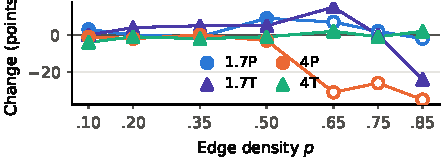
\includegraphics[width=\columnwidth]{fig_addstats.pdf}
\caption{What adding clustering and RWSE to the same degrees changes on node degree (all three statistics minus the degree primer, points), per arm and density. Hollow as in Figure~\ref{fig:headroom}.}
\label{fig:addstats}
\end{figure}

\paragraph{Filler and fragile questions (\S\ref{sec:side}).} A primer changes $38$-$69\%$ of the questions filler changes and $3$-$15\%$ of the rest. % [overlap]
Some questions are fragile: on plain Qwen3-1.7B's node degree, $24$ of $400$ change outcome when the same prompt is generated again. Every condition changes them far more often than the rest ($46$-$67\%$ against $14$-$26\%$, $q\leq.018$). Yet they carry only $11$ to $16$ of each condition's $65$ to $113$ changes, a lower bound on chance with only two generations per prompt. % [rerunflip]
Where accuracy without a primer is $25$-$75\%$, components, clustering and RWSE average $+1.6$ points while filler averages $-6.9$ on the same cells. % [fillerband]

\begin{table}[!t]
\centering\footnotesize\setlength{\tabcolsep}{4pt}
\begin{tabular}{llrrr}
\toprule
Arm & Primer & Raw & Balanced & Yes\\
\midrule
1.7P & none & 70.50 & 79.86 & 56.2\\ % [eemain] (%)
 & degree & 74.50 & 82.30 & 51.7\\ % [eemain] (%)
 & clustering & 74.25 & 82.42 & 52.5\\ % [eemain] (%)
 & RWSE & 75.50 & 82.68 & 50.1\\ % [eemain] (%)
 & all & 82.00 & \textbf{87.71} & 44.8\\ % [eemain] (%)
 & components & 62.25 & \textbf{74.23} & 64.5\\ % [eemain] (%)
 & filler & 54.75 & \textbf{69.11} & 72.0\\ % [eemain] (%)
\addlinespace[2pt]
1.7T & none & 99.00 & 99.02 & 27.1\\ % [eemain] (%)
 & degree & 96.50 & 97.61 & 29.9\\ % [eemain] (%)
 & clustering & 98.00 & 98.63 & 28.6\\ % [eemain] (%)
 & RWSE & 97.75 & 98.17 & 28.3\\ % [eemain] (%)
 & all & 97.25 & 98.12 & 29.5\\ % [eemain] (%)
 & components & 98.25 & 98.81 & 28.3\\ % [eemain] (%)
 & filler & 98.50 & 98.68 & 27.8\\ % [eemain] (%)
\addlinespace[2pt]
4P & none & 90.50 & 93.22 & 35.7\\ % [eemain] (%)
 & degree & 85.75 & \textbf{90.27} & 40.7\\ % [eemain] (%)
 & clustering & 94.50 & \textbf{96.25} & 32.3\\ % [eemain] (%)
 & RWSE & 80.50 & \textbf{86.69} & 46.3\\ % [eemain] (%)
 & all & 80.50 & \textbf{86.69} & 46.1\\ % [eemain] (%)
 & components & 87.75 & 91.64 & 39.0\\ % [eemain] (%)
 & filler & 83.50 & \textbf{88.74} & 43.2\\ % [eemain] (%)
\addlinespace[2pt]
4T & none & 99.75 & 99.83 & 26.8\\ % [eemain] (%)
 & degree & 99.75 & 99.83 & 26.8\\ % [eemain] (%)
 & clustering & 99.00 & 99.32 & 27.0\\ % [eemain] (%)
 & RWSE & 98.50 & 98.68 & 26.9\\ % [eemain] (%)
 & all & 98.75 & 99.15 & 27.1\\ % [eemain] (%)
 & components & 99.25 & 99.49 & 27.0\\ % [eemain] (%)
 & filler & 99.75 & 99.83 & 26.8\\ % [eemain] (%)
\bottomrule
\end{tabular}
\caption{Edge existence, main sweep ($400$ prompts per row): raw and balanced accuracy over all prompts and the share of finished answers that say yes, all in \%. Truncation is in Table~\ref{tab:truncmatrix}. Bold: balanced accuracy differs from the same arm without a primer (paired permutation, BH $q<.05$ within arm).} % [eemain]
\label{tab:ee}
\end{table}

\begin{table}[!t]
\centering\footnotesize
\setlength{\tabcolsep}{1.6pt}
\begin{tabular}{llrrrrrr}
\toprule
 & & Correct & \multicolumn{3}{c}{Cycle named} & \multicolumn{2}{c}{No cycle}\\
\cmidrule(lr){4-6}\cmidrule(l){7-8}
Arm & Primer & ``yes'' & Real & Invented & Not a & All & Edge\\
 & & ($n$) & & & cycle & & count\\
\midrule
1.7P & none & 363 & 36.9 & 43.5 & 16.0 & 3.6 & 0.8\\ % [ccanswer] [cctest]
 & degree & 293 & \textbf{13.0} & \textbf{20.5} & 1.4 & 65.2 & 55.6\\ % [ccanswer] [cctest]
 & clustering & 397 & 39.5 & 48.1 & 7.8 & 4.5 & 1.0\\ % [ccanswer] [cctest]
 & RWSE & 362 & 33.7 & 40.3 & 19.9 & 6.1 & 1.7\\ % [ccanswer] [cctest]
 & all & 391 & 38.4 & 50.4 & 7.9 & 3.3 & 1.3\\ % [ccanswer] [cctest]
 & components & 371 & \textbf{27.8} & 40.4 & 25.3 & 6.5 & 4.3\\ % [ccanswer] [cctest]
 & filler & 375 & 33.3 & \textbf{55.5} & 9.6 & 1.6 & 0.0\\ % [ccanswer] [cctest]
\addlinespace[2pt]
1.7T & none & 388 & 79.9 & 17.8 & 1.0 & 1.3 & 0.5\\ % [ccanswer] [cctest]
 & degree & 301 & \textbf{61.5} & \textbf{29.6} & 0.0 & 9.0 & 9.0\\ % [ccanswer] [cctest]
 & clustering & 386 & 80.6 & 19.2 & 0.0 & 0.3 & 0.3\\ % [ccanswer] [cctest]
 & RWSE & 397 & \textbf{68.0} & 20.7 & 10.6 & 0.8 & 0.5\\ % [ccanswer] [cctest]
 & all & 385 & 73.0 & 21.8 & 3.1 & 2.1 & 1.8\\ % [ccanswer] [cctest]
 & components & 358 & 74.9 & 22.6 & 0.0 & 2.5 & 2.0\\ % [ccanswer] [cctest]
 & filler & 400 & 77.2 & 19.8 & 2.5 & 0.5 & 0.0\\ % [ccanswer] [cctest]
\addlinespace[2pt]
4P & none & 396 & 34.1 & 23.0 & 6.8 & 36.1 & 25.0\\ % [ccanswer] [cctest]
 & degree & 387 & \textbf{13.4} & \textbf{3.9} & 2.1 & 80.6 & 65.6\\ % [ccanswer] [cctest]
 & clustering & 398 & \textbf{48.7} & \textbf{31.2} & 1.0 & 19.1 & 5.8\\ % [ccanswer] [cctest]
 & RWSE & 395 & 33.2 & 20.8 & 38.7 & 7.3 & 0.5\\ % [ccanswer] [cctest]
 & all & 395 & \textbf{45.1} & \textbf{33.4} & 6.6 & 14.9 & 0.8\\ % [ccanswer] [cctest]
 & components & 388 & 39.2 & 18.6 & 3.4 & 38.9 & 26.5\\ % [ccanswer] [cctest]
 & filler & 394 & \textbf{44.2} & 28.2 & 5.3 & 22.3 & 2.3\\ % [ccanswer] [cctest]
\addlinespace[2pt]
4T & none & 397 & 96.5 & 3.3 & 0.0 & 0.3 & 0.0\\ % [ccanswer] [cctest]
 & degree & 375 & \textbf{90.9} & 5.1 & 0.0 & 4.0 & 2.7\\ % [ccanswer] [cctest]
 & clustering & 397 & 95.5 & 4.5 & 0.0 & 0.0 & 0.0\\ % [ccanswer] [cctest]
 & RWSE & 398 & \textbf{55.0} & 2.5 & 42.5 & 0.0 & 0.0\\ % [ccanswer] [cctest]
 & all & 395 & 92.7 & 6.3 & 0.0 & 1.0 & 1.0\\ % [ccanswer] [cctest]
 & components & 384 & \textbf{92.2} & 4.4 & 0.0 & 3.4 & 2.9\\ % [ccanswer] [cctest]
 & filler & 399 & 94.2 & 5.0 & 0.5 & 0.3 & 0.0\\ % [ccanswer] [cctest]
\bottomrule
\end{tabular}
\caption{What the correct cycle-check answers rest on (main sweep; every correct answer is ``yes''). \emph{Correct ($n$)}: count of correct, finished answers; the other columns are \% of those $n$, and Real, Invented, Not a cycle and All sum to 100. \emph{Real}: every step of the cycle is an edge; \emph{Invented}: a step is not an edge; \emph{Not a cycle}: a length-2 or retraced walk. \emph{Edge count}: the answers under All that argue from the number of edges, identified by their wording. The valid arguments are Real and Edge count, which is valid because $40$ nodes with at least $40$ edges must contain a cycle. Bold (Real, Invented only): differs from the same model without a primer (paired, BH $q<.05$).} % [ccanswer] [cctest]
\label{tab:cycles}
\end{table}


\begin{table*}[t]
\centering\scriptsize
\setlength{\tabcolsep}{3.4pt}
\begin{tabular}{llrrrrrrr}
\toprule
Task & Arm & none & degree & clustering & RWSE & all & components & filler\\
\midrule
Degree & 1.7P & 0.00 & $+0.0$ & $+0.0$ & $+0.2$ & $+0.0$ & $+0.0$ & $+0.0$\\ % [main] [trunc]
 & 1.7T & 0.75 & $+4.5$ & $-0.5$ & $+0.0$ & $-0.5$ & $-0.2$ & $-0.5$\\ % [main] [trunc]
 & 4P & 0.00 & $+0.0$ & $+0.0$ & $+0.0$ & $+0.0$ & $+0.0$ & $+0.0$\\ % [main] [trunc]
 & 4T & 2.75 & $-2.5$ & $-2.0$ & $-0.5$ & $-1.0$ & $-0.5$ & $-1.8$\\ % [main] [trunc]
\addlinespace[2pt]
Neighbors & 1.7P & 0.00 & $+0.0$ & $+0.0$ & $+0.0$ & $+0.2$ & $+0.0$ & $+0.0$\\ % [main] [trunc]
 & 1.7T & 1.25 & $+0.2$ & $-1.0$ & $-0.8$ & $-0.5$ & $-0.2$ & $-0.8$\\ % [main] [trunc]
 & 4P & 0.00 & $+0.0$ & $+0.0$ & $+0.0$ & $+0.0$ & $+0.0$ & $+0.0$\\ % [main] [trunc]
 & 4T & 3.25 & $-0.2$ & $+1.2$ & $-0.2$ & $+1.0$ & $+0.2$ & $-0.5$\\ % [main] [trunc]
\addlinespace[2pt]
Edge count & 1.7P & 29.75 & $-20.2$ & $-11.8$ & $-11.8$ & $-1.8$ & $-2.5$ & $-3.5$\\ % [main] [trunc]
 & 1.7T & 81.75 & $-0.8$ & $+0.8$ & $+5.0$ & $-12.2$ & $+0.5$ & $+1.2$\\ % [main] [trunc]
 & 4P & 0.00 & $+1.8$ & $+0.2$ & $+0.5$ & $+0.8$ & $+0.8$ & $+0.0$\\ % [main] [trunc]
 & 4T & 79.50 & $-20.8$ & $-26.0$ & $-12.2$ & $-23.8$ & $-25.0$ & $-13.0$\\ % [main] [trunc]
\addlinespace[2pt]
Edge exists & 1.7P & 0.00 & $+0.0$ & $+0.0$ & $+0.2$ & $+0.0$ & $+0.0$ & $+0.0$\\ % [main] [trunc]
 & 1.7T & 0.25 & $+0.2$ & $+0.0$ & $+0.0$ & $-0.2$ & $+0.0$ & $-0.2$\\ % [main] [trunc]
 & 4P & 0.00 & $+0.5$ & $+0.0$ & $+0.0$ & $+0.2$ & $+0.0$ & $+0.0$\\ % [main] [trunc]
 & 4T & 0.25 & $+0.0$ & $+0.8$ & $+1.2$ & $+1.0$ & $+0.5$ & $+0.0$\\ % [main] [trunc]
\midrule
Node count & 1.7P & 0.00 & $+0.0$ & $+0.0$ & $+0.0$ & $+0.0$ & $+0.0$ & $+0.0$\\ % [main] [trunc]
 & 1.7T & 7.75 & $-5.0$ & $-7.8$ & $-7.8$ & $-7.8$ & $-0.5$ & $-7.8$\\ % [main] [trunc]
 & 4P & 0.00 & $+0.0$ & $+0.0$ & $+0.0$ & $+0.0$ & $+0.0$ & $+0.0$\\ % [main] [trunc]
 & 4T & 0.00 & $+0.2$ & $+0.2$ & $+0.2$ & $+0.0$ & $+0.0$ & $+0.0$\\ % [main] [trunc]
\addlinespace[2pt]
Cycle & 1.7P & 9.00 & $+8.2$ & $-8.2$ & $-7.2$ & $-8.0$ & $-2.5$ & $-2.8$\\ % [main] [trunc]
 & 1.7T & 3.00 & $+21.2$ & $+0.5$ & $-2.2$ & $+0.8$ & $+7.5$ & $-3.0$\\ % [main] [trunc]
 & 4P & 0.75 & $+0.8$ & $-0.2$ & $+0.5$ & $-0.2$ & $+0.8$ & $+0.5$\\ % [main] [trunc]
 & 4T & 0.75 & $+4.8$ & $+0.0$ & $-0.2$ & $+0.5$ & $+3.2$ & $-0.5$\\ % [main] [trunc]
\bottomrule
\end{tabular}
\caption{Complete main-sweep truncated shares: no-primer baseline (percent of all prompts) and paired changes (percentage points), for the same queries as Table~\ref{tab:full}. Each of its cells' \emph{wrong} share equals $100\%$ minus its correct and truncated shares. P/T: plain/thinking; components and filler are diagnostics. No significance marks are assigned to truncation contrasts.} % [setup] [main]
\label{tab:truncmatrix}
\end{table*}


\paragraph{Side statistics (\S\ref{sec:side}).} On edge existence, every primer that moves balanced accuracy does so in a plain arm (bold in Table~\ref{tab:ee}). Plain Qwen3-4B's false alarms also climb with shared neighbors, from $0.2\%$ of non-edges with none to $38.8\%$ with four or more. % [eeshared]
At high density the statistics barely vary within a graph: printed clustering values have SD $0.021$ at $p=.65$, and rounded RWSE takes $3.3$ distinct value pairs per graph at $p=.50$, against $12.5$ distinct degrees. Gains there, such as clustering's $+11.3$ on dense plain Qwen3-4B's node degree with its procedure unchanged, are presentation effects. % [cluster] [rwse] [clusthi] [clustproc]

\paragraph{Against the thinking mode (\S\ref{sec:vsthink}).} Equivalence in Table~\ref{tab:vsthink} rests on $90\%$ intervals. The component sentence's gap on plain Qwen3-4B's neighbor sets lies in $[-2.0,+2.5]$, inside the $\pm3$-point margin. The degree primer's gap on plain Qwen3-1.7B's neighbor sets is not significant ($q=.24$), but its interval reaches $+6.2$, so the two are not shown to be level. % [vsthink] [vsequiv]

\paragraph{Thinking mode (\S\ref{sec:thinkmode}).} Thinking models check stated values against their own count. Under the degree primer, thinking Qwen3-1.7B still lists the neighbors in $90\%$ of responses at $p\geq.35$, and thinking Qwen3-4B ends on the stated value in $93\%$ of its conflicts. % [verify] [pdsource]
In the follow-ups, clustering gains thinking Qwen3-1.7B $2.5$ points at $p\leq.50$ ($q=.043$) and loses $5.4$ at $p\geq.65$ ($q=.0015$), where filler loses $11.4$. % [ddthink]
Of the answers a condition changes, $44$-$65\%$ for thinking Qwen3-1.7B and $83$-$95\%$ for thinking Qwen3-4B involve a response that ran out of tokens. % [churnwhy]

\paragraph{What responses rest on (\S\ref{sec:reston}).} Clustering and RWSE change the share of queries answered right on both degree and neighbor set with $q\geq.16$ in every arm. The degree primer lowers it for plain Qwen3-4B and raises it for plain Qwen3-1.7B, from $54.0\%$ to $62.5\%$. % [joint]
Table~\ref{tab:cycles} classifies every correct, finished cycle-check answer by the argument it cites. The degree primer raises the plain valid shares from $34.2\%$ and $58.5\%$ to $50.2\%$ and $76.5\%$, and truncation accounts for $21.2$ of the $21.8$ points it costs thinking Qwen3-1.7B but only $8.2$ of the $17.5$ it costs plain Qwen3-1.7B (Tables~\ref{tab:full} and~\ref{tab:truncmatrix}). RWSE, all three statistics and filler lower plain Qwen3-4B's valid share to $33.2\%$, $45.2\%$ and $45.8\%$ ($q<.05$). % [ccvalid] [main] [trunc]

\paragraph{Node count.} The encoding's first line lists the $40$ node ids, so node count measures which number a model writes, not reading. Plain Qwen3-1.7B answers $39$, the last id, on $68.5\%$ of finished responses without a primer and on $1.2\%$ under clustering, hence Table~\ref{tab:full}'s large node-count effects. % [nodecount] [ncanswer]

\section{Pilot and the Clustering Screen}
\label{app:pilot}
\paragraph{Pilot.} On the published GraphQA graphs ($5$-$19$ nodes), Gemma~4 E4B/12B and Qwen3-8B/14B, each in plain and thinking mode, were near ceiling without a primer on most tasks; only edge count separated them. This is why the main study uses 40-node graphs and smaller models.

\paragraph{The clustering effect.} Clustering on plain Qwen3-1.7B's node degree emerged from a $40$-cell screen, so Table~\ref{tab:clust} tests it on graphs the screen did not see, on a fresh seed, against filler, on 20-160-node graphs at fixed mean degree, at high density and on Qwen3-8B. It shows little sign of using the stated values. No response mentions clustering, and the gain does not depend on the queried node's printed coefficient ($p=.5$). Components and filler also cut the neighbors the model misses ($0.94$ and $1.05$ per response at $p=.35$-$.50$, against $0.86$ with clustering and $1.49$ with none). % [rqbehaviour] [rqhetero]

\begin{table}[!t]
\centering\scriptsize
\setlength{\tabcolsep}{4pt}
\begin{tabular}{lrl}
\toprule
Test & Gain & $p$ or $q$\\
\midrule
Screened graphs ($700$) & $+1.29$ & $p=.47$\\ % [ddplain] [ddrep] [rqselection] [ddplainfill] [fixdeg8]
Unscreened graphs ($2{,}100$) & $+2.1$ & $p=.031$\\ % [ddplain] [ddrep] [rqselection] [ddplainfill] [fixdeg8]
$p\leq.50$ ($1{,}600$ pairs) & $+3.8$ & $q=.0035$\\ % [ddplain] [ddrep] [rqselection] [ddplainfill] [fixdeg8]
Fresh seed & $+4.2$ & $p=.00055$ ($.022$ corr.)\\ % [ddplain] [ddrep] [rqselection] [ddplainfill] [fixdeg8]
Against filler & $+3.2$ & $q=.014$\\ % [ddplain] [ddrep] [rqselection] [ddplainfill] [fixdeg8]
Fixed mean degree ($3{,}200$) & $+6.2$ & $q<.001$\\ % [fixdeg17]
$p\geq.65$ ($1{,}200$ pairs) & $-0.7$ & $q=.57$\\ % [ddplain] [ddrep] [rqselection] [ddplainfill] [fixdeg8]
Qwen3-8B ($3{,}200$) & $-1.0$ & $q=.05$\\ % [ddplain] [ddrep] [rqselection] [ddplainfill] [fixdeg8]
\bottomrule
\end{tabular}
\caption{The clustering effect on node degree against no primer (against filler where the row says so), in points, for plain Qwen3-1.7B except the last row, which is Qwen3-8B. \emph{Screened}: graphs the screen also used; \emph{fixed mean degree}: the 20-160-node grid. \emph{corr.}: Bonferroni over the screen's cells.}
\label{tab:clust}
\end{table}

\end{document}
